\documentclass[11pt,a4paper]{article}

\usepackage{blindtext}
\usepackage[margin=1in]{geometry}
\usepackage{xcolor} %use color
\definecolor{mygreen}{rgb}{0,0.6,0}
\definecolor{mygray}{rgb}{0.5,0.5,0.5}
\definecolor{mymauve}{rgb}{0.58,0,0.82}
\usepackage{listings}
\renewcommand{\lstlistingname}{Codebeispiel}
\lstset{ %
  backgroundcolor=\color{white}, % choose the background color; you must add \usepackage{color} or \usepackage{xcolor}
  basicstyle=\footnotesize, % the size of the fonts that are used for the code
  breakatwhitespace=false, % sets if automatic breaks should only happen at whitespace
  breaklines=true, % sets automatic line breaking
  commentstyle=\color{mygreen}, % comment style
  extendedchars=true, % lets you use non-ASCII characters; for 8-bits encodings only, does not work with UTF-8
  keepspaces=true, % keeps spaces in text, useful for keeping indentation of code (possibly needs columns=flexible)
  keywordstyle=\color{blue}, % keyword style
  stringstyle=\color{orange}, % string literal style
  tabsize=2, % sets default tabsize to 2 spaces
}
\lstdefinelanguage{JavaScript}{
  morekeywords=[1]{break, continue, delete, else, for, function, if, in,
    new, return, this, typeof, var, void, while, with},
  % Literals, primitive types, and reference types.
  morekeywords=[2]{false, null, true, boolean, number, undefined,
    Array, Boolean, Date, Math, Number, String, Object},
  % Built-ins.
  morekeywords=[3]{eval, parseInt, parseFloat, escape, unescape},
  sensitive,
  morecomment=[s]{/*}{*/},
  morecomment=[l]//,
  morecomment=[s]{/**}{*/}, % JavaDoc style comments
  morestring=[b]',
  morestring=[b]"
}[keywords, comments, strings]
\lstset{
  language=JavaScript,
  extendedchars=true,
  basicstyle=\footnotesize\ttfamily,
  showstringspaces=false,
  showspaces=false,
  numbers=left,
  numberstyle=\footnotesize,
  numbersep=5pt,
  tabsize=2,
  breaklines=true,
  showtabs=false,
  captionpos=b
}

\usepackage[ngerman]{babel}
\usepackage[autostyle=true,german=quotes]{csquotes}
\usepackage[sfdefault]{roboto}
\usepackage{hyperref}

\usepackage{microtype}
\usepackage{hyphenat}
\hyphenation{Mathe-matik wieder-gewinnen}

\usepackage{graphicx}
\usepackage{subcaption}
\usepackage{pdflscape}

\usepackage{multicol}

\makeatletter         
\renewcommand\maketitle{
{\raggedright % Note the extra {
\begin{center}
{\Huge \bfseries \sffamily \@title }\\[2ex] 
\@author\\[1ex] 
\@date, Hochschule der Medien, Stuttgart\\[1ex]
\end{center}}} % Note the extra }
\makeatother

\title{Optimierung einer VueJS-Webseite: Ladezeitenreduktion}
\author{Andreas Nicklaus, an067, 44835}

\begin{document}
\maketitle

\tableofcontents

\section{Vorstellung des Projekts}
Diese Hausarbeit behandelt die Optimierung einer VueJS-Webseite im Rahmen des Seminars \enquote{Entwicklung von Rich Media Systemen} unter dem Motto \enquote{Web Performance Optimizations}.
Zu diesem Zweck wurden mehrere Änderungen an einer bereits bestehenden Webseite vorgenommen, die mit VueJS entwickelt wurde.

Die Webseite in diesem Projekt ist eine Marketingwebseite für das Onlinetool für Physiotherapiepraxen namens \enquote{Leto}.
Die Webseite ist strikt getrennt von der Anwendung, umfasst aber mehrere Admin-Tools und die Nutzerkontenverwaltung.
Die Kommunikation mit dem Backend-Server erfolgt über HTTP und ist für dieses Projekt nahezu vollkommen irrelevant.

Gehostet wird die Webseite auf einer kostenlosen und minimal ausgestatteten AWS EC2 Instanz und mithilfe von Docker.
Auf der Host-Maschine läuft zusätzlich auf Docker ein NGINX-Proxy-Manager Container, der die Requests über die Domain \enquote{leto.andreasnicklaus.de} an den richtigen Container weiterleitet.
Die Erstellung des Docker-Images erfolgt automatisiert in Github Actions und hat folgende relevante Build-Schritte:

\begin{enumerate}
  \item Installation der zum Buildprozess notwendigen Pakete (apt-get und npm)
  \item Kopieren der Source-Dateien
  \item Bauen der Webseite mittels \verb|npm run build|
  \item Wechseln auf NGINX-alpine Docker Image
  \item Kopieren der NGINX-Konfigurationsdatei
  \item Kopieren der gebauten Webseite auf den NGINX-Webserver
\end{enumerate}

Auf der Grundlage dieser Webseite, Entwicklungsumgebung und dieses Deployments werden im Folgenden Schwachstellen gesucht, Verbesserungsmöglichkeiten umrissen, deren Umsetzung beschrieben und Effekt ausgewertet.
Zielsetzung dabei ist es, die Performance der Webseite im Allgemeinen zu verbessern, ohne den Aufwand für die Weiterentwicklung zu vergrößern oder die Größe des Dockerimages und somit der Speicheranforderungen an den Webserver zu vergrößern.

\section{Testfall und Tools}
Um die Performance der Webseite sowie den Effekt der Verbesserungsversuche zu bewerten, werden in diesem Kapitel die genutzten Testtools und die beachteten Metriken beschrieben.

\subsection{Tool A: WebPageTest}\label{subsec:WebPageTest}
Das erste Tool, das zur Auswertung der Performance genutzt wurde, ist das Onlinetool WebPageTest, das unter \href{https://www.webpagetest.org}{www.webpagetest.org} erreichbar ist.
WebPageTest wurde von Patrick Meenan als internes Evaluationswerkzeug für AOL entwickelt und ist sein 2008 frei verfügbar.

Mithilfe von WebPageTest können Ladezeiten, Verarbeitungsperformance und weitere Vergleichsmaßstäbe festgehalten, bzw. erstellt werden.
Dabei wird hoher Wert darauf gelegt, den Programm- und Datenflow des Clients zu visualisieren und insbesondere zeitlich aufzudröseln.
Der größte Faktor, der für die Verwendung in diesem Projekt ausschlaggebend war, ist die Tatsache, dass jeder Test eine eindeutige ID hat, mit der die Testergebnisse nachvollziehbar gespeichert werden und mit der mehrere Tests miteinander verglichen werden können.

Zusätzlich bietet das Tool die Möglichkeit, optional bei Tests einen Lighthousetest (s. \hyperref[subsec:Lighthouse]{Lighthouse Chrome Extension} und \hyperref[subsec:PageSpeed]{PageSpeed Insights}) und einen Carbon Control Test mitlaufen zu lassen, der den Kohlenstoffausstoß des Seitenaufrufs abschätzt.
Außerdem werden weitere hilfreiche Tools wie ein Bildanalysetool, eine Request-Map und ein Sicherheitscheck direkt verlinkt.
Im Rahmen dieser Arbeit werden lediglich die integrierten Ladeanalysen, der integrierte Lighthouse Report, die Ladezeitvisualisierung \enquote{Filmstrip}, der \enquote{Content Breakdown} und das externe Bildanalysetool verwendet.

\subsection{Tool B: PageSpeed Insights}\label{subsec:PageSpeed}
Ebenso wie WebPageTest ist auch PageSpeed Insights ein frei verfügbares Onlinetool zur Auswertung der Performance einer Webseite.
Allerdings wird hier kaum Wert auf die Auswertung des Renderverhaltens der Webseite gelegt, sondern ein Lighthousetest durchgeführt. Das heißt, dass statische Tests in 4 Kategorien durchgeführt werden: Performance, Barrierefreiheit, Best Practices und Suchmaschinenoptimierung (SEO).
Für dieses Projekt wird lediglich der Performance Report ausgewertet.

Der Performance Report gibt eine Bewertung zwischen 0 und 100 ab, der sich aus 5 Metriken zusammensetzt, die sich wiederum aus vielen Messungen ergeben:

\begin{enumerate}
  \item Der First Contentful Paint (FCP) gibt an, wie lange das Rendering dauert, bis das erste Element auf der Benutzeroberfläche angezeigt wird.
  Es ist somit ein Maß dafür, wie lange die Auswertung und das Laden der Ressourcen dauert, bevor das Rendering des HTMLs beginnen kann.
  \item Der Largest Contentful Paint (LCP) beschreibt das Ende des Renderings und gibt an, wie lange es gedauert hat, bis das letzte HTML-Element gerendert wurde.
  Der LCP ist somit unter anderem ein Maß für die maximale Größe von gerenderten Dateien oder Elementen oder für Animationen, die die Fertigstellung des Renderings verzögern.
  \item Die Total Blocking Time (TBT) ist die Zeit zwischen FCP und \enquote{Time To Interactive} (TTI, dt.: Zeit zur Interaktivität).
  Für Benutzerfreundlichkeit sowie analytische Auswertung des Nutzerverhaltens ist diese Metrik besonders wichtig, da der Gedankengang und das Verhalten des Nutzers durch eine hohe TBT verzögert wird.
  Ausgelöst kann eine hohe TBT durch langes Laden, Parsen und Ausführen von JavaScript, insb. bei ineffizientem Code.
  \item Der Cumulative Layout Shift (CLS) misst die Bewegung von sichtbaren Elementen in der Nutzeransicht. Auch dieser Wert ist maßgeblich für die Benutzerfreundlichkeit und das effektive Nutzerverhalten auf der Webseite.
  Der CLS wird von langsam nachladenden HTML-Elementen oder durch fehlende Größenangaben von Elementen verursacht, die widerrum das Verschieben von anderen Elementen bewirken.
  \item Der Speed Index (SI) gibt an, wie schnell Inhalte während des Ladens visuell dargestellt werden. SI ist damit eine Metrik, die das sofortige Anzeigen von Elementen belohnt.
  SI ist allerdings auch eine Metrik, die den Effekt von allen Bestandteilen der Webseite zusammenfasst und ist deshalb nicht immer ohne Wissen über den Sourcecode gut nachvollziehbar. 
\end{enumerate}

Im Rahmen dieser Arbeit wird PageSpeed Insights lediglich verwendet, um einen Vergleichs-, bzw. Bestätigungswert als \enquote{zweite Meinung} für den Lighthouse Report von WebPageTest und Erklärungen zu den Ergebnissen zu bekommen, weil die Performance je nach Zustand des Servers und Clients zwischen Ausführungen der Tests schwanken kann.

\subsection{Tool C: Lighthouse Chrome Extension}\label{subsec:Lighthouse}
Die Google Chrome Extension \href{https://chromewebstore.google.com/detail/lighthouse/blipmdconlkpinefehnmjammfjpmpbjk}{Lighthouse} ist eine Erweiterung für den Browser Google Chrome und wurde von Google entwickelt.
Mit dessen Hilfe können Lighthouse Reports lokal für im Browser geöffnete Seiten erstellt werden und bereits in der Entwicklungsphase manuell generiert werden.
Die Auswertungen sind dabei dieselben wie bei \hyperref[subsec:WebPageTest]{WebPageTest} und \hyperref[subsec:PageSpeed]{PageSpeed Insights}.

Ebenso wie PageSpeed Insights wird die Lighthouse Chrome Extension im Rahmen dieser Arbeit bloß verwendet, um einen weiteren Vergleichswert für den Performance-Score zu bekommen und um bei der Entwicklung die Verbesserungen zu testen.

\subsection{Metriken und Maße}
Für die Evaluierung der Testergebnisse durch die oben genannten Tools wurden die vielen Messwerte reduziert auf 9 Metriken, deren Entwicklung während des Optimierungsprozesses hier interessant sind.
Dazu gehören von WebPageTest die \enquote{Page Weight} (dt.: Seitengewicht), die die Größe der geladenen Dateien in Bytes angibt, der LCP und SI (von hier an zur Unterscheidung mit \enquote{WPT LCP} und \enquote{WPT SI} abgekürzt).
Von den Lighthouse Reports werden der generelle Performance-Score (LH Score) sowie der FCP, LCP, SI, CLS und TTI ausgewertet.

\section{Verbesserungsschritte}
Tabelle~\ref{tab:versionen} zeigt die 12 Versionen, die in dieser Arbeit verglichen werden.
Neben der Version v00, die die Version vor Projektbeginn bezeichnet, und den Versionen v03 und v04, die keine Performanceoptimierungsschritte, sondern lediglich inhaltliche Updates beinhalten, gibt es 9 Versionsschritte, die 5 Bestandteile der Webseite optimieren.
Die folgenden Unterkapitel beschreiben die Versionsschritte und die Webseitbestandteile, die in den Versionen optimiert werden.

Im Folgekaptitel~\ref{sec:experimente} wird beschrieben, wie die Versionen ausgewertet und welche Performanceverbesserungen dadurch erzielt wurden.

\subsection{Prerendering}
Die Version v01 führt als ersten Schritt ein, dass die Seiten vorgerendert werden.
Mit Vue wird usprünglich ein HTML-Skelett geladen, dass mittels JavaScript mit Inhalten gefüllt wird.
Deshalb muss der Browser in diesem Prozess erst das HTML-Skelett laden, anschließend den verlinkten JavaScript-Chunk-Vendor laden, der auf die relevanten JavaScript- und CSS-Dateien verweist.
Erst, wenn all diese Dateien geladen werden, kann der Browser die Seite rendern.
Das ist oft effizient, weil das initiale HTML sehr klein ist und das Navigieren zwischen Seiten weniger Ladeaufwand hat.
Dieses Verfahren ist lediglich beim ersten Laden der Seite aufwendig, weil viele Dateien in sog. Chained Requests geladen werden.

Im Prerendering werden die Vue-Templates, die mittels Vue-Router einem Pfad zugewiesen werden, einmalig im Build-Prozess der Seite zusammengefügt und gerendert.
So kann das HTML, das im allerersten Request empfangen wird, gleich mit Inhalten gefüllt werden, die im Browser sofort gerendert werden.

\begin{lstlisting}[language=JavaScript, caption={Implementierung des Single Page Prerenderings}, label={lst:prerender}]
new PrerenderSpaPlugin({
  staticDir: path.join(__dirname, 'dist'),
  routes: routes.filter(r => r.meta?.prerender).map(r => r.path),
  renderer: new PrerenderSpaPlugin.PuppeteerRenderer({
    inject: {},
    renderAfterElementExists: '[data-view]',
  }),
  postProcess: (renderedRoute) => {
    renderedRoute.html = renderedRoute.html
      .replace(/<script (.*?)>/g, '<script $1 defer>')
      .replace('id="app"', 'id="app" data-server-rendered="true"');

    return renderedRoute;
  }
})
\end{lstlisting}

Das Codebeispiel~\ref{lst:prerender} zeigt die Implementierung mithilfe des NPM-Packages PrerenderSpaPlugin.
Das Plugin nutzt den PuppeteerRenderer, der in einem Headless Chrome die Seite öffnet und rendert.
Sobald ein HTML-Element mit dem Attribut \enquote{data-view} vorhanden ist, speichert das Plugin das HTML der Seite ab.
Deshalb muss das Vue-Template der View das Attribut \verb|data-view| bekommen.

Zusätzlich wurde in diesem Schritt jedes verlinkte Skript mit dem Attribut \enquote{defer} versehen, damit es dem Rendering nicht im Weg steht, und die App wird als prerendered annotiert. 
Durch diesen Schritt können alle statischen Inhalte sofort nach Laden und Parsen des HTML gerendert werden und die Rendering-Engine muss nicht auf das Laden der JavaScript-Dateien warten.
Da dies nur bei den öffentlich zugänglichen und statischen Seiten sinnvoll ist, werden nur diese Seiten vorgerendert.
Diese Eigenschaft wird durch für jede Route händisch festgelegt (s. Codebeispiel~\ref{lst:prerender}, Zeile 3).

\subsection{Render-Blocking Stylesheets}
Die zweite Hürde, die für schnelles Rendering der Seite genommen wurde, ergibt sich aus der Reihenfolge, in der Dateien geladen und geparst werden.
Das HTML wird top-down (dt.: von oben nach unten) geparst und die verlinkten Ressourcen i.d.R. auch in dieser Reihenfolge geladen, bevor das Parsing und Rendering des HTML weiterläuft.
Elemente und Ressourcen müssen daher explizit verzögert geladen werden.
Bei JavaScript kann das entweder dadurch erreicht werden, dass Script-Tags ans Ende des HTML-Bodys gestellt oder mit dem defer-Attribut ausgezeichnet werden.
Zweiteres wird in v01 automatisiert erledigt (s. Codebeispiel~\ref{lst:prerender}, Zeile 10).

Bei Stylesheets (CSS) gibt es keine Möglichkeit, das verzögerte Laden so simpel umzusetzen.
Stattdessen werden ab Version v02 die Stylesheets mit dem Attribut \verb|rel="preload"| vorgeladen und nach dem Laden wird das Attribut auf \verb|rel="stylesheet"| geändert.
Da diese Funktionalität auf JavaScript basiert, wird das Stylesheet zusätzlich in einem \verb|noscript|-Tag klassisch eingebunden (s. Codebeispiel~\ref{lst:stylesheets}). 
Damit wird nicht die Ladereihenfolge der Ressourcen geändert, aber die Rendering-Engine wartet nicht mehr darauf, dass das Stylesheet geladen wurde, um das Rendering fortzusetzen.

\begin{lstlisting}[language=html, caption={Entfernte Render-Blocking Stylesheets (\enquote{\$1} steht für den jeweiligen Quellpfad für das Stylesheet)}, label={lst:stylesheets}]
<link rel="preload" href="$1" as="style" onload="this.onload=null;this.rel='stylesheet'">
<noscript>
  <link rel="stylesheet" href="$1">
</noscript>
\end{lstlisting}

Zur Optimierung des CSS gehört außerdem, dass externe Stylesheet nicht in den internen verwiesen werden, da das Laden derer sonst erst nach dem Parsen der internen Stylesheets beginnen würde.
Stattdessen müssen alle externen Stylesheets bereits im HTML-Head verlinkt werden.
In diesem Projekt tritt das nur auf das Laden der Roboto-Schriftart zu.
Codebeispiel~\ref{lst:chained} zeigt, wie im Vue-Template das Stylesheet von Google-Servern verlinkt wird.
Diese Verlinkung landet nach dem Build in den internen Stylesheets für das Template.
Codebeispiel~\ref{lst:unchained} zeigt die Einbindung in die index.html ab Version v05, die im Build-Prozess automatisiert \enquote{unchained} eingebunden wird (s. Codebeispiel~\ref{lst:stylesheets}).

\begin{lstlisting}[language=html, caption={Chained Request im Vue-Template}, label={lst:chained}]
<style lang="scss">
  @import url("https://fonts.googleapis.com/css2?family=Roboto&display=swap");
</style>
\end{lstlisting}
\begin{lstlisting}[language=html, caption={\enquote{Un-Chained} Request im HTML (index.html)}, label={lst:unchained}]
<link
  rel="stylesheet"
  href="https://fonts.googleapis.com/css2?family=Roboto&display=swap"
/>
\end{lstlisting}

\subsection{Bildoptimierung}\label{subsec:images}
Die Versionen v05 und v06 beinhalten hauptsächlich Optimierungen bezüglich der Bytegröße und der Pixelgröße der verwendeten Bilder.
Bis v05 wurden alle Bilder als \verb|img|-Tag eingebunden und bis auf das Brand-Logo und ein Hintergrundbild (SVG) sind alle Bilder im WebP-Format in Originalgröße verlinkt.
Die Darstellungsgröße dieser Bilder auf dem Bildschirm wurde bis dahin lediglich über CSS bestimmt.
\pagebreak

\begin{lstlisting}[language=html, caption={Einbindung von Bildern als picture-Tag}, label={lst:images}]
<picture>
  <source
    :srcset="`${appleDevices_avif_1} 200w, ${appleDevices_avif_2} 783w,
      ${appleDevices_avif_3} 1123w, ${appleDevices_avif} 1920w`"
    sizes="(max-width: 768px) 100vw, 50vw"
  />
  <source
    :srcset="`${appleDevices_webp_1} 200w, ${appleDevices_webp_2} 783w,
      ${appleDevices_webp_3} 1123w, ${appleDevices_webp} 1920w`"
    sizes="(max-width: 768px) 100vw, 50vw"
  />
  <img :src="appleDevices_webp" ... />
</picture>
\end{lstlisting}

Das Codebeispiel~\ref{lst:images} zeigt die Einbindung von Bildern im \verb|picture|-Tag mit mehreren Bildgrößen und Bildformaten.
Es wird davon ausgegangen, dass jeder Browser heute entweder Bilder im AVIF-Format oder WebP-Format darstellen kann.
Aus diesem Grund werden zwei Sourcesets definiert, die jeweils die Bilder in 4 verschiedenen Breiten (200px, 780px, 1123px und 1920px) anbieten.
Außerdem wird direkt im HTML mit angegeben, welche Breite das Bild im HTML haben wird (s. Zeilen 5 und 10), damit der Browser das passende Bild laden kann.

Dadurch wird bewirkt, dass der Browser selbst entscheiden kann, welche Pixelgröße und welches Format geladen werden soll.
Version v06 ändert die Verteilung der 4 Bildgrößen zu einer feineren und linearen Verteilung mit 6 Bildweiten: 320px, 640px, 960px, 1280px, 1600px und 1920px.
Diese Bildgrößen passen zudem besser mit handelsüblichen Endgeräten zusammen, da die Bilder auf dieser Seite entweder 50\% oder 100\% der Bildschirmweite einnehmen.   

\subsection{JS-Optimierungen}
Für die Version v07 hat eine Untersuchung ergeben, dass ein sehr großer Teil des JavaScripts von Bootstrap-Icons eingenommen werden (s. Abbildung \ref{fig:treemap}).

\begin{figure}[h]
  \centering
  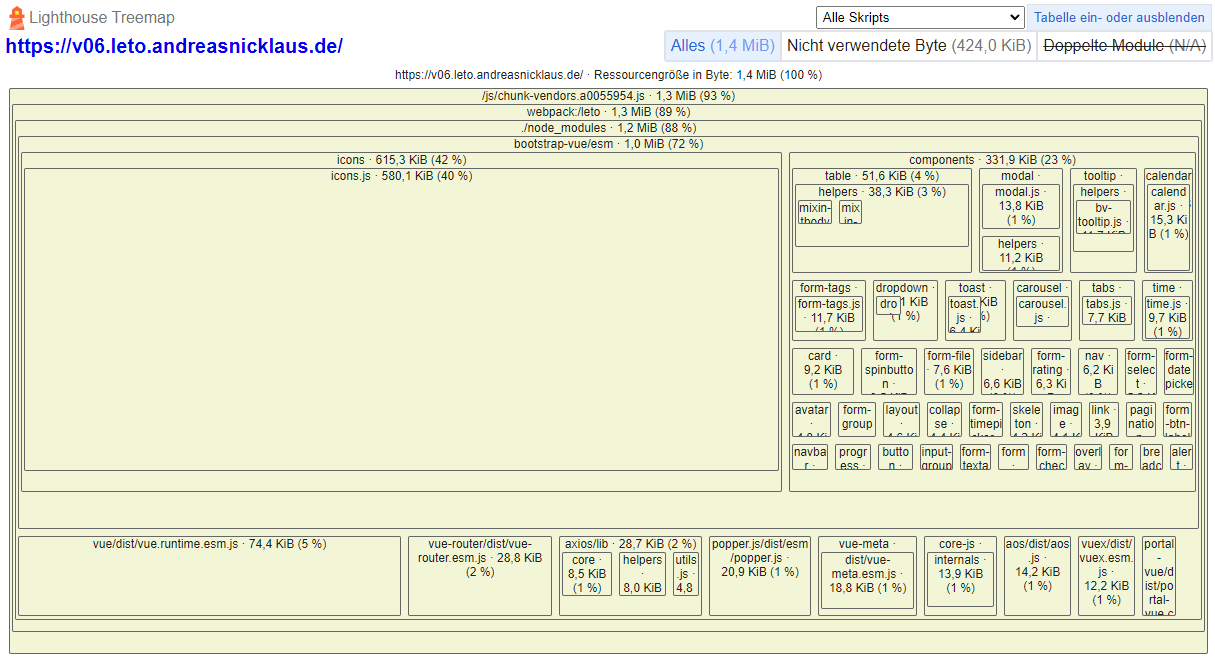
\includegraphics[scale=.5]{images/v06_treemap.png}
  \caption{Strukturkarte des JavaScripts in Version v06: 40\% des JavaScripts werden durch Bootstrap-Icons eingenommen.}
  \label{fig:treemap}
\end{figure}

Aus diesem Grund wurde in v07 lediglich eine Änderung vorgenommen: Da sehr viele Bootstrap-Icons importiert werden, von denen aber nur wenige verwendet werden, werden jetzt lediglich die Icons importiert, die auf der Seite auch verwendet werden.
Codebeispiel~\ref{lst:icons} zeigt, wie die Icons importiert und als Komponenten registriert werden.

\begin{lstlisting}[language=JavaScript, caption={Epliziter Import und Einbindung von Bootstrap-Icons}, label={lst:icons}]
// vorher: alle Icons werden importiert und eingebunden
// import { BootstrapVueIcons } from 'bootstrap-vue'
// Vue.use(BootstrapVueIcons)

import { BootstrapVue, BIconBoxArrowUpRight, BIconPerson, ... } from 'bootstrap-vue'
Vue.component("b-icon-box-arrow-up-right", BIconBoxArrowUpRight)
Vue.component("b-icon-person", BIconPerson)
  ...
\end{lstlisting}

Diese Art von manuellem Treeshaking verringert die Größe des JavaScripts von Bootstrap auf die wirklich notwendigen Elemente.

Außerdem haben erste Untersuchungen gezeigt, dass viel JavaScript geladen wird, das nicht verwendet wird.
Deshalb wird in der Version v08 mit dem Optimieren der JS-Chunks experimentiert.
Webpack bietet dafür bereits eine Möglichkeit an, die maximale Größe von JavaScript-Dateien festzulegen.
Mithilfe dessen wird ein Maximum für die Dateigröße festgelegt und die Anzahl der generierten Chunks dynamisch festgelegt.
Das Codebeispiel~\ref{lst:chunks} zeigt die Konfiguration für diese Optimierung.

\begin{lstlisting}[language=JavaScript, caption={Konfiguration von Webpack zur Limitierung der Chunkgröße}, label={lst:chunks}]
configureWebpack: (config) => {
  config.optimization = {
    runtimeChunk: 'single',
    splitChunks: {chunks: 'all', maxInitialRequests: Infinity, maxSize: 500000}
  }
}
\end{lstlisting}

\subsection{Timing}
Diese letzte Rubrik an Optimierungsschritten umfasst das Experimentieren mit dem Timing der Darstellung von Elementen.
Die Version v09 entfernt alle Animationen von der Startseite, die mittels des NPM-Pakets \enquote{Animate On Scroll} (AOS) Elemente erst erscheinen lässt, wenn sie in der Ansicht des Nutzers auftauchen.
Die Versionen v10 und v11 fügt zu \verb|img|-Tags das Attribut \verb|loading="lazy"| hinzu.
Lazy-Loading bedeutet, dass die Bilder erst geladen werden, wenn der Client für nötig erachtet, beispielsweise wenn das Bild kurz außerhalb der Ansicht des Nutzers ist und vielleicht gleich in die Ansicht gescrollt wird.

\section{Experimente und Analyse}\label{sec:experimente}
Um die Versionen zu testen, wurden alle Versionen als eigenen Dockerimage erstellt und auf demselben Host als getrennte Dockercontainer deployt.
Anschließend wurde der NGINX-Proxy-Manager so konfiguriert, dass die Container unter der jeweiligen Versionsnummer online erreichbar sind.
Somit ist beispielweise die Version v00 unter \href{https://v00.leto.andreasnicklaus.de}{v00.leto.andreasnicklaus.de} erreichbar.

So konnten alle Versionen mit WebPageTest getestet und miteinander verglichen werden.

\subsection{Testergebnisse}
Tabelle~\ref{tab:versionen} zeigt die rohen Ergebnisse aus den mit WebPageTest ausgeführten Tests.
Dabei ist auffällig, dass das Prerendering der Version v01 direkt Verbesserungen allen Messwerten außer der Page Weight und der TTI bringt.
Ebenso positiv auffällig ist das Einführen von Bildern im AVIF-Format und den Responsive Image Sizes in der Version v05, die insbesondere Verbesserungen im SI, der Page Weight (s. Abbildung~\ref{fig:PageWeight}) und der TTI (s. Abbildung~\ref{fig:TTI}) gebracht haben.

Hinweis: Da die Tests mit allen Tools starken Schwankungen bis zu 20\% unterliegen, sind kleine Verschlechterungen oder Verbesserungen in einzelnen Versionen nicht zu beachten, wenn die Veränderung nicht in den Folgeversionen Bestand behält.

\begin{figure}[h]
  \begin{subfigure}{.5\textwidth}
    \centering
    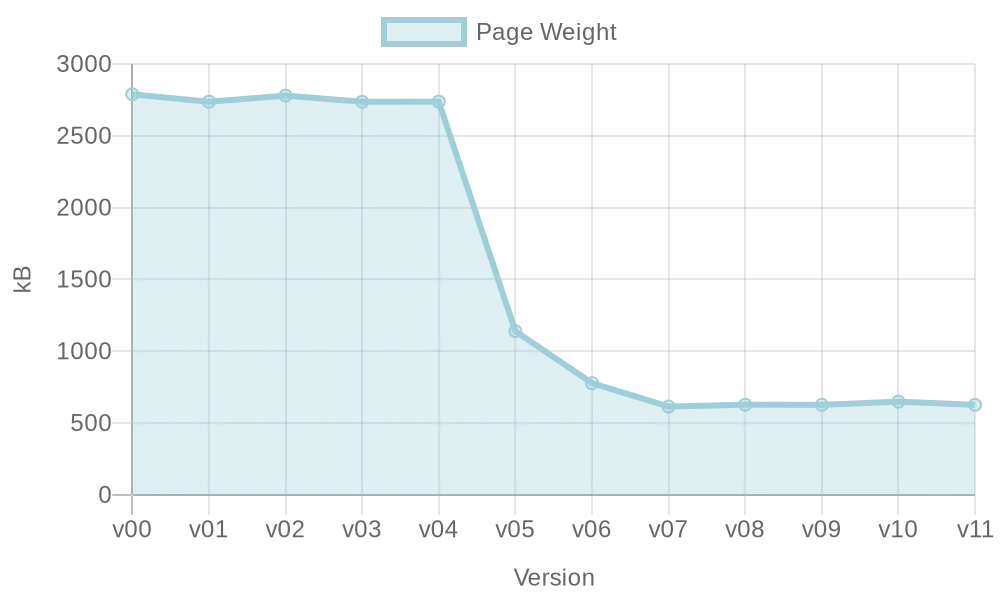
\includegraphics[width=.8\linewidth]{images/PageWeight.png}
    \caption{Page Weight der Startseite pro Version in kB}
    \label{fig:PageWeight}
  \end{subfigure}%
  \begin{subfigure}{.5\textwidth}
    \centering
    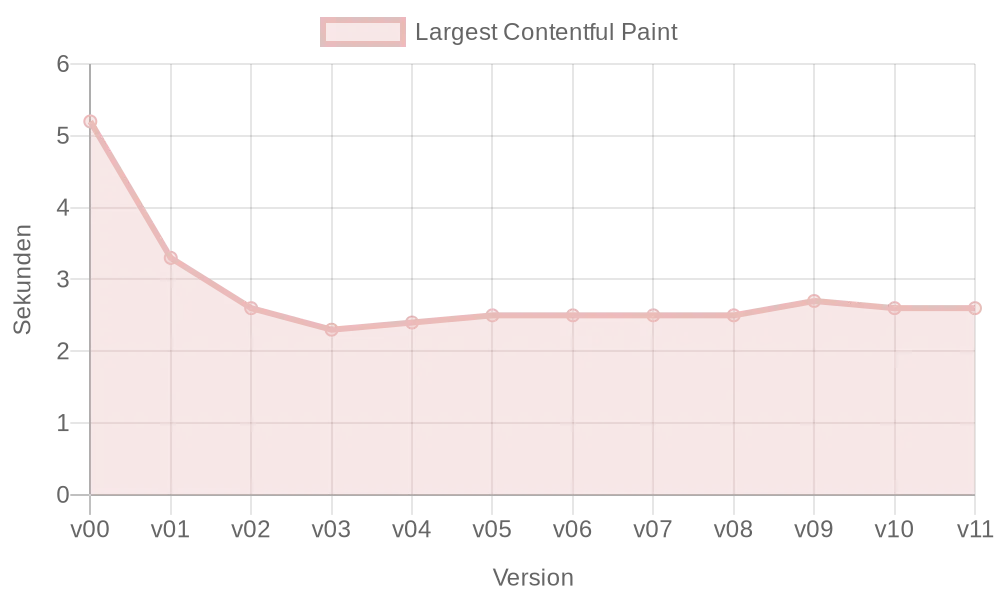
\includegraphics[width=.8\linewidth]{images/LCP.png}
    \caption{LCP der Startseite in Sekunden}
    \label{fig:LCP}
  \end{subfigure}
  \begin{subfigure}{.5\textwidth}
    \centering
    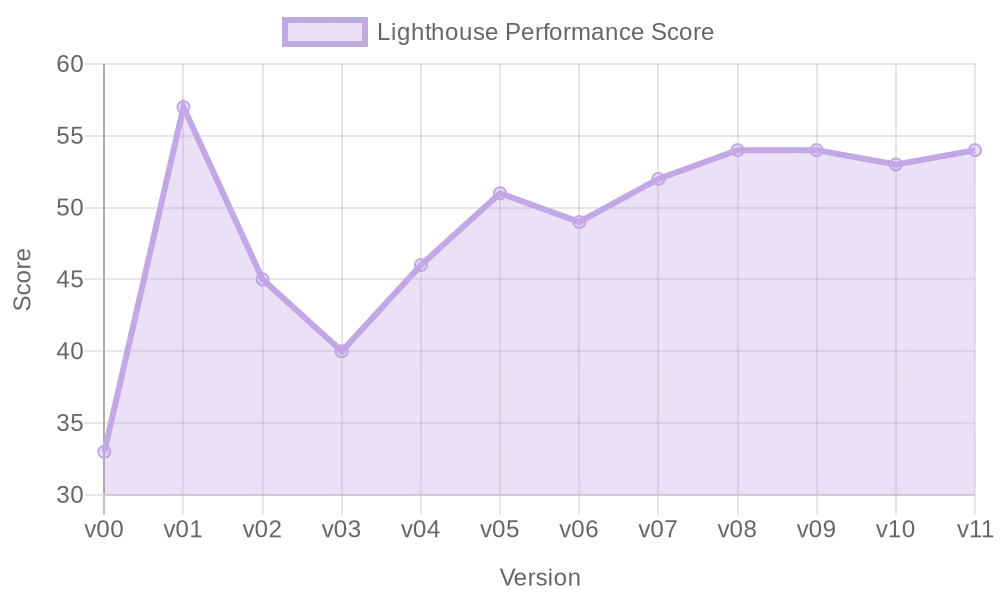
\includegraphics[width=.8\linewidth]{images/LH Score.png}
    \caption{Lighthouse Performance-Score der Startseite}
    \label{fig:LHScore}
  \end{subfigure}
  \begin{subfigure}{.5\textwidth}
    \centering
    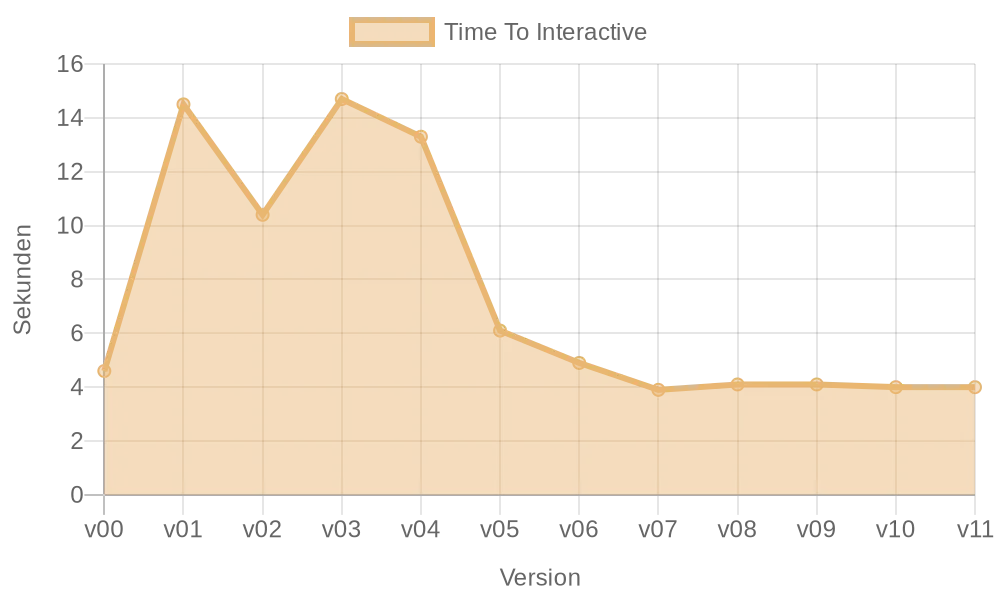
\includegraphics[width=.8\linewidth]{images/TTI.png}
    \caption{TTI der Startseite in Sekunden}
    \label{fig:TTI}
  \end{subfigure}
  \caption{Performance der Startseite je Version}
  \label{fig:performance}
\end{figure}

\subsection{Interpretation}
Die Abbildung~\ref{fig:content} vergleicht die Größe der Seite nach Dateityp vor dem Projekt (v00) und nach dem Projekt (v11).
Die Seitengröße wurde von 2789 kB auf 627 kB (-77,5\%) reduziert (vgl. Abbildung~\ref{fig:PageWeight}).
2063 kB der eingesparten 2162 kB wurden alleine durch die Verkleinerung der Bilder eingespart (von ca. 2100 kB auf 35,8 kB für Bilder).
Daraus lässt sich zumindest für dieses Projekt darauf schließen, dass das Laden der Bilder für die Seitengröße das größte Potenzial für Verbesserungen hatte.

Ebenso können wir beobachten, dass das Prerendering der statischen Seiten das HTML zwar um ca. 17 kB vergrößert, aber den FCP, die Ladezeiten für verlinkte Ressourcen (LCP und SI) und dadurch den Lighthouse Performance-Score beachtlich verbessert.
Diese zwei Optimierungsschritte haben sich als die besten Optimierungsschritte herausgestellt.

\begin{figure}[h]
  \begin{subfigure}{.5\textwidth}
    \centering
    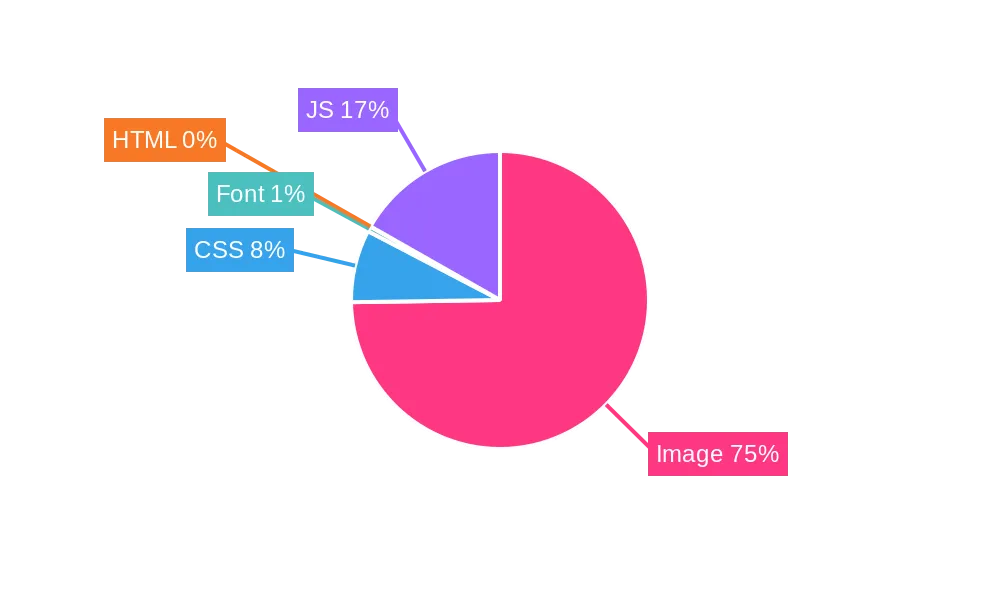
\includegraphics[width=.8\linewidth]{images/v00_content.png}
    \caption{Version v00}
    \label{fig:v00content}
  \end{subfigure}%
  \begin{subfigure}{.5\textwidth}
    \centering
    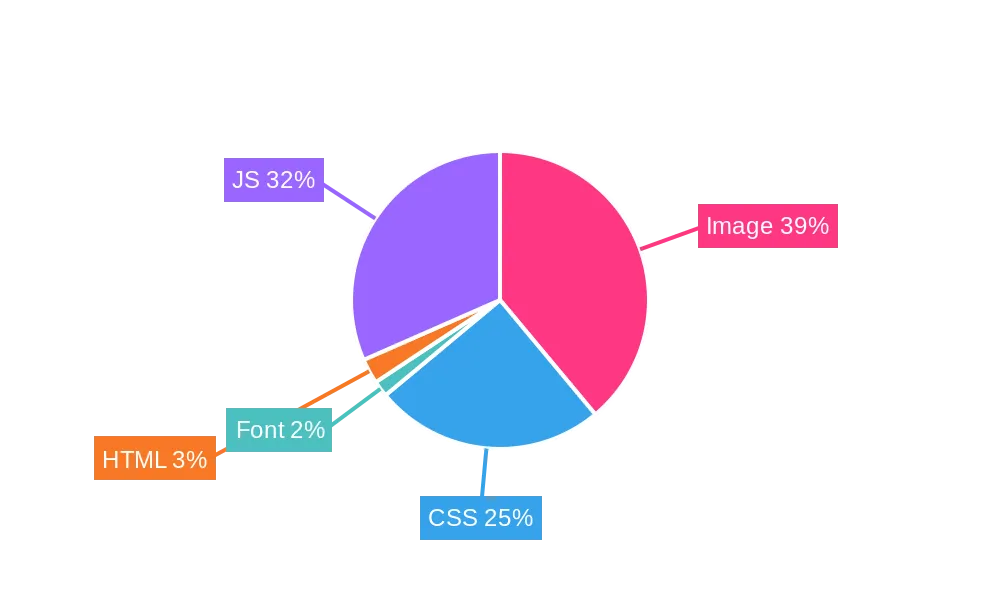
\includegraphics[width=.8\linewidth]{images/v11_content.png}
    \caption{Version v11}
    \label{fig:v11content}
  \end{subfigure}
  \caption{Vergleich der Dateitypen bzgl. der unkomprimierten Bytegröße zwischen den Versionen v00 (insg.: 2789 kB) und v11 (insg.: 627 kB)}
  \label{fig:content}
\end{figure}

\section{Fazit}
Das Projekt hat gezeigt, dass sich die Optimierung einer VueJS-Webseite von der Optimierung einer statischen Webseite nur in einem Punkt unterscheidet: Die Verbesserung des Nutzererlebnisses, das sich durch Single-Page-Applications ergibt, schadet der Performance beim ersten Laden der Seite durch Chained Requests.
Dieser Unterschied lässt sich durch Prerendering weitestgehend ausbessern und erlaubt es Entwicklern, weitere Schritte oder Kontrollen des Build-Prozesses zu automatisieren.

Diese automatisierten Schritte unterscheiden sich von der Optimierung einer statischen HTML-Seite nicht.
In diesem Beispielfall haben das Entfernen von ungebrauchtem JavaScript und die Bildoptimierung neben dem Prerendering die besten Ergebnisse erzielt.

Um dieses Projekt weiterzuführen, lassen sich mehrere Punkte abzeichnen, die sich sowohl aus dem Lighthouse Report als auch aus Image Lintern ergeben.
Das Treeshaking, das sich durch das manuelle Entfernen von ungenutztem JavaScript als erfolgreich herausgestellt hat, könnte man noch weiter optimieren und auf das Entfernen von ungenutztem CSS, sog. \enquote{CSS-Pruning}, und das Trennen von nach dem Laden ausgeführten JavaScript ausweiten.
Ebenso müsste das Potenzial von Preloading der LCP-Ressource genauer untersucht werden sowie der Performance-Unterschied von unterschiedlichen Hostingarchitekturen und -konfigurationen.
Als letzter Punkt wäre ein interessantes Projekt der Umgang mit Bildern, die im Original in einer kleinen Größe vorliegen, aber auf großen Bildschirmen eine hohe Auflösung haben sollen.

Insgesamt ist das Projekt ein Erfolg, da die Rahmenbedingungen bzgl. Speicherplatz und Rechenleistung eingehalten wurden, die Performance verbessert wurde und die Ladezeiten aufgrund geringerer Page Weight deutlich verringert wurden.

\appendix
\section{Tabellen}

\begin{table}[h]
  \begin{tabular}{|l|l|}
    \hline
    \textbf{Versionsbezeichnung} & \textbf{Änderungsbeschreibung}\\
    \hline
    v00 & -- (Ursprungsversion vor Projektbeginn)\\
    \hline
    v01 & Prerendering für statische Seiten\\
    \hline
    v02 & Render-Blocking Stylesheets entfernt\\
    \hline
    v03 & Updated Docker Build Workflow\\
    \hline
    v04 & Verbessertes Access Management\\
    \hline
    v05 & AVIF-Bilder, Chained Request für Fonts entfernt\\
    \hline
    v06 & Lineare Verteilung der Bildgrößen\\
    \hline
    v07 & Import nur der genutzten Icons anstelle von allen\\
    \hline
    v08 & JS-Chunks gesplittet\\
    \hline
    v09 & Animationen entfernt\\
    \hline
    v10 & Alle Bilder werden lazy-loaded\\
    \hline
    v11 & Zuerst sichtbare SVGs werden lazy-loaded\\
    \hline
  \end{tabular}
  \caption{Versionsnummerierungen und die Änderungen, die in der Version neu hinzugekommen sind. Hinweis: Versionen v03 und v04 haben inhaltliche Änderungen an der Webseite, beinhalten aber keinen Performanceoptimierungsschritt.}\label{tab:versionen}
\end{table}

\begin{landscape}
\begin{table}[h]
  \begin{tabular}{|l|l|l|l|l|l|l|l|l|l|}
    \hline
    \textbf{Version} & \textbf{Page Weight (kB)} & \textbf{WPT LCP (ms)} & \textbf{WPT SI (ms)} & \textbf{LH Score} & \textbf{FCP (ms)} & \textbf{LCP (ms)} & \textbf{SI (ms)} & \textbf{TTI (ms)} & \textbf{CLS} \\
    \hline
    v00 & 2789 kB & 4736 ms & 5970 ms & 33 & 4600 ms & 5200 ms & 7500 ms & 4600 ms & 0,751 \\
    \hline
    v01 & 2737 kB & 2964 ms & 4368 ms & 57 & 3300 ms & 3300 ms & 5100 ms & 14500 ms & 0 \\
    \hline
    v02 & 2780 kB & 1877 ms & 2936 ms & 45 & 900 ms & 2600 ms & 5500 ms & 10400 ms & 0,936 \\
    \hline
    v03 & 2737 kB & 1888 ms & 6297 ms & 40 & 900 ms & 2300 ms & 5600 ms & 14700 ms & 0,936 \\
    \hline
    v04 & 2738 kB & 1804 ms & 6019 ms & 46 & 900 ms & 2400 ms & 4100 ms & 13300 ms & 0,936 \\
    \hline
    v05 & 1140 kB & 1891 ms & 2813 ms & 51 & 900 ms & 2500 ms & 2500 ms & 6100 ms & 0,78 \\
    \hline
    v06 & 778 kB & 1898 ms & 2957 ms & 49 & 900 ms & 2500 ms & 3200 ms & 4900 ms & 0,781 \\
    \hline
    v07 & 612 kB & 1896 ms & 2930 ms & 52 & 900 ms & 2500 ms & 3200 ms & 3900 ms & 0,781 \\
    \hline
    v08 & 628 kB & 2029 ms & 2306 ms & 54 & 900 ms & 2500 ms & 2700 ms & 4100 ms & 0,78 \\
    \hline
    v09 & 627 kB & 2189 ms & 2068 ms & 54 & 900 ms & 2500 ms & 2600 ms & 4100 ms & 0,78 \\
    \hline
    v10 & 649 kB & 2342 ms & 2165 ms & 53 & 900 ms & 2600 ms & 2500 ms & 4000 ms & 0,78 \\
    \hline
    v11 & 627 kB & 2218 ms & 2122 ms & 54 & 900 ms & 2600 ms & 2500 ms & 4000 ms & 0,78 \\
    \hline
  \end{tabular}
  \caption{Rohergebnisse der WebPageTest-Ergebnisse pro Version. Hinweis: Die rohen Werte unterliegen bei mehrfacherer Testausführung starken Schwankungen (bis zu 20\% in beide Richtungen).}\label{tab:versionen}
\end{table}

\section*{Was sonst keinen Platz gefunden hat: Bilddateigrößen und Bildformate}
\begin{multicols}{2}
  Neben den in dieser Arbeit beschriebenen Optimierungsergebnissen wurde eine weitere Beobachtung gemacht, die sonst keinen Platz gefunden hätte.
  Bei der Untersuchung von Dateigrößen im Vergleich zur Pixelgröße ist aufgefallen, dass sich WebP und AVIF unterschiedlich verhalten, wenn die Pixelgröße verändert wird.
  \href{https://quickchart.io/chart?w=400&h=400&c=%7B%0A%20%20type%3A%20%27line%27%2C%0A%20%20data%3A%20%7B%0A%20%20%20%20labels%3A%20%5B%0A%20%20%20%20%20%20%27Original%20(1900%20px)%27%2C%0A%20%20%20%20%20%20%27%401%20(1600%20px)%27%2C%0A%20%20%20%20%20%20%27%402%20(1280%20px)%27%2C%0A%20%20%20%20%20%20%27%403%20(960%20px)%27%2C%0A%20%20%20%20%20%20%27%404%20(640%20px)%27%2C%0A%20%20%20%20%20%20%27%405%20(320%20px)%27%2C%0A%20%20%20%20%5D%2C%0A%20%20%20%20datasets%3A%20%5B%0A%20%20%20%20%20%20%7B%0A%20%20%20%20%20%20%20%20label%3A%20%27PNG%27%2C%0A%20%20%20%20%20%20%20%20data%3A%20%5B689%2C2747%2C1743%2C972%2C443%2C130%5D%2C%0A%20%20%20%20%20%20%20%20backgroundColor%3A%20%27%23c4a7e755%27%2C%0A%20%20%20%20%20%20%20%20borderColor%3A%20%27%23c4a7e7%27%2C%0A%20%20%20%20%20%20%7D%2C%0A%20%20%20%20%20%20%7B%0A%20%20%20%20%20%20%20%20label%3A%20%27WebP%27%2C%0A%20%20%20%20%20%20%20%20data%3A%20%5B126%2C71%2C56%2C41%2C23%2C10%5D%2C%0A%20%20%20%20%20%20%20%20backgroundColor%3A%20%27%230400ff55%27%2C%0A%20%20%20%20%20%20%20%20borderColor%3A%20%27%230400ff%27%2C%0A%20%20%20%20%20%20%7D%2C%0A%20%20%20%20%20%20%7B%0A%20%20%20%20%20%20%20%20label%3A%20%27AVIF%27%2C%0A%20%20%20%20%20%20%20%20data%3A%20%5B374%2C36%2C28%2C20%2C13%2C6%5D%2C%0A%20%20%20%20%20%20%20%20backgroundColor%3A%20%27%23ffaa0055%27%2C%0A%20%20%20%20%20%20%20%20borderColor%3A%20%27%23ffaa00%27%2C%0A%20%20%20%20%20%20%7D%2C%0A%20%20%20%20%5D%2C%0A%20%20%7D%2C%0A%20%20options%3A%20%7B%0A%20%20%20%20scales%3A%20%7B%0A%20%20%20%20%20%20xAxes%3A%20%5B%7B%20scaleLabel%3A%20%7B%20display%3A%20true%2C%20labelString%3A%20%27Bildbreite%27%20%7D%20%7D%5D%2C%0A%20%20%20%20%20%20yAxes%3A%20%5B%7B%20scaleLabel%3A%20%7B%20display%3A%20true%2C%20labelString%3A%20%27kB%27%20%7D%20%7D%5D%2C%0A%20%20%20%20%7D%2C%0A%20%20%7D%2C%0A%7D}
  {Diese Grafik} veranschaulicht, wie sich die Dateigröße eines Beispielbildes in den Formaten PNG, WebP und AVIF verhält, wenn die Pixelgröße mit dem NPM-Paket \enquote{sharp} gemäß der in Kapitel~\ref{subsec:images} beschriebenen Größen verkleinert wird.
  Diese Untersuchung findet in der Arbeit keine Beachtung und ist deshalb hier getrennt von der Arbeit.
\end{multicols}

\end{landscape}
  
\end{document}